% Evidence: analyses/028-2026-09-20-70m-optimized-grid/observations/001-matched-70m-grid.md.
% Figure/data: Analysis028/02_figures.py; data/full-trained-results.json.
% Optimization: Run042 retained controls; Run045 matched grid; Analysis028 observations/001-matched-70m-grid.md.
\section{Experimental study}
\label{sec:experiments}

We pretrain Pythia-14M, 70M, and 410M from random initialization~\citep{biderman2023pythia} on MiniPile~\citep{kaddour2023minipile}. Each run receives 712 optimizer steps and 1.493 billion input tokens. Within each size, runs share initialization, data order and training budget. We evaluate loss and $\Smodel$ on the full validation set. Appendix~\ref{app:experiment} gives the full protocol. %For comparison, we apply TEAL-style post-hoc magnitude thresholding~\citep{liu2024teal} at $a,m,h,z$, using percentile targets $p=0,0.1,\ldots,0.9$. Site--layer thresholds are calibrated separately on ten training blocks.

% \textbf{Experiments across model sizes.}
% We use 14M for extensive intervention ablations and kernel development, and use 70M as a scale check of whether the observed sparse structures remain exploitable after adapting the implementation. We also evaluated 410M, but it operates in a different optimization regime, exhibiting higher loss than 70M and a larger gradient norm after the same token budget. Because these effects are not isolated, our detailed intervention and runtime analyses focus on 14M and 70M. Appendix~\ref{app:410m-results} reports the 410M results, and Figure~\ref{fig:a0-optimization} shows the corresponding training trajectories.

% \textbf{Agentic kernel development.}
% We used Codex with GPT-6 Astra~\citep{openaigpt6astra} to develop specialized GPU kernels under human guidance, starting from the implementation of \citet{cetin2026sparser} and adapting it to Pythia. Candidate changes were tested on a fixed subset of training sequences, and the selected implementation was fixed before evaluation. We then checked full-validation outputs against numerical tolerances and timed a fixed subset of sequences. Appendix~\ref{app} gives the execution paths, correctness checks, and timing protocol. This case illustrates how agentic coding can make execution tests practical for a representation-learning study.


% Evidence: Analysis028 observations/001-matched-70m-grid.md; 01_collect.py and 02_figures.py.
% Later endpoint: Analysis030 observations/001-later-70m-endpoint.md; 01_integrate.py and 02_plot.py.
% Original 14M development: Run029 observations/06-implementation-and-claim-audit.md.
% Clipping latency: Run036 results/clipping-final-kernel.json.
% Argument and claim audit: reviews/2026-09-21-results-arc/README.md.
% \subsection{From sparsity to speedups}

\subsection{Extensive ablations at 14M}
% Evidence: analyses/033-2026-09-21-14m-latency-quality-frontier/observations/006-threshold-tables.md.
% Values: data/frontier.json, generated by Analysis033/01_plot.py; ceilings: Table~\ref{tab:interventions}.

We compare interventions at 14M, separating aggressive thresholding ($\kappa=0.5$) from moderate settings ($\kappa=\{0.05,0.1\}$). First, \textbf{broader coverage increases attainable sparsity without consistently reducing latency.} At $\kappa=0.5$, $T_7/P_{\mathrm{all}}$ more than doubles the sparsity of $T_4/P_{\mathrm{all}}$ (27.48\% versus 12.71\%) at 0.473 versus 0.459\,ms (Table~\ref{tab:14m-aggressive}). Within $T_7$, broadening pressure from $P_h$ to $P_{\mathrm{all}}$ adds 10.82 percentage points of sparsity with nearly unchanged latency, while loss rises from 5.732 to 5.829. All seven aggressive recipes reduce latency relative to Base but increase loss.

\begin{table}[!htbp]
\centering\small
\setlength{\tabcolsep}{7pt}
\caption{\textbf{Sparsity and latency under aggressive thresholding.} All seven thresholded 14M recipes at $\kappa=0.5$. All latencies, including Base, use the specialized 14M kernel on RTX\,5090 (BF16, batch one, 2,048 tokens, full logits), with three timing processes per checkpoint.}
\label{tab:14m-aggressive}
\begin{tabular}{@{}lrrrr@{}}
\toprule
Recipe & Ceiling (\%) & Sparsity (\%) & Latency (ms) & Loss \\
\midrule
Base (kernel) & 0.00 & 0.00 & 0.652 & 5.209 \\
\midrule
$T_2/P_h$ & 5.35 & 5.34 & 0.506 & 5.536 \\
\midrule
$T_4/P_0$ & 12.83 & 10.22 & 0.479 & 5.660 \\
$T_4/P_h$ & 12.83 & 10.23 & 0.462 & 5.723 \\
$T_4/P_{\mathrm{all}}$ & 12.83 & 12.71 & 0.459 & 6.038 \\
\midrule
$T_7/P_0$ & 29.95 & 15.39 & 0.479 & 5.703 \\
$T_7/P_h$ & 29.95 & 16.66 & 0.474 & 5.732 \\
$T_7/P_{\mathrm{all}}$ & 29.95 & 27.48 & 0.473 & 5.829 \\
\bottomrule
\end{tabular}
\end{table}

\textbf{Moderate thresholding with local pressure offers a better quality--latency balance.}
At both moderate thresholds, $P_h$ gives lower loss and latency than $P_{\mathrm{all}}$ under both $T_4$ and $T_7$ (Table~\ref{tab:14m-moderate}). At $\kappa=0.05$, $T_4/P_h$ reaches 0.562\,ms with loss 5.196, versus Base's 0.652\,ms and 5.209. Narrowing thresholding to $T_2/P_h$ improves loss further to 5.134.

\begin{table}[!htbp]
\centering\small
\setlength{\tabcolsep}{7pt}
\caption{\textbf{Quality--latency trade-offs at moderate thresholds.} All seven thresholded 14M recipes at $\kappa\in\{0.05,0.1\}$, with the same metrics and timing protocol as Table~\ref{tab:14m-aggressive}.}
\label{tab:14m-moderate}
\begin{tabular}{@{}lrrrrr@{}}
\toprule
Recipe & $\kappa$ & Ceiling (\%) & Sparsity (\%) & Latency (ms) & Loss \\
\midrule
Base (kernel) & --- & 0.00 & 0.00 & 0.652 & 5.209 \\
\midrule
\multirow{2}{*}{$T_2/P_h$} & 0.05 & 5.35 & 5.00 & 0.590 & 5.134 \\
 & 0.1 & 5.35 & 5.17 & 0.573 & 5.151 \\
\midrule
\multirow{2}{*}{$T_4/P_0$} & 0.05 & 12.83 & 8.21 & 0.630 & 5.434 \\
 & 0.1 & 12.83 & 8.95 & 0.593 & 5.420 \\
\midrule
\multirow{2}{*}{$T_4/P_h$} & 0.05 & 12.83 & 9.04 & 0.562 & 5.196 \\
 & 0.1 & 12.83 & 9.34 & 0.529 & 5.229 \\
\midrule
\multirow{2}{*}{$T_4/P_{\mathrm{all}}$} & 0.05 & 12.83 & 10.46 & 0.573 & 5.490 \\
 & 0.1 & 12.83 & 11.39 & 0.534 & 5.548 \\
\midrule
\multirow{2}{*}{$T_7/P_0$} & 0.05 & 29.95 & 9.13 & 0.635 & 5.438 \\
 & 0.1 & 29.95 & 10.43 & 0.594 & 5.429 \\
\midrule
\multirow{2}{*}{$T_7/P_h$} & 0.05 & 29.95 & 10.13 & 0.575 & 5.195 \\
 & 0.1 & 29.95 & 10.90 & 0.542 & 5.237 \\
\midrule
\multirow{2}{*}{$T_7/P_{\mathrm{all}}$} & 0.05 & 29.95 & 9.86 & 0.635 & 5.463 \\
 & 0.1 & 29.95 & 11.80 & 0.593 & 5.429 \\
\bottomrule
\end{tabular}
\end{table}


\subsection{Spillover: Local pressure induces nonlocal sparsity}
\label{sec:paired-results}
% Evidence: Analysis021/pressure-scope/observations/O017-layer-sparsity-style.md;
% plot_layer_sparsity.py and data/layer-sparsity-review.json.
% Geometry: Analysis024/observations/039-ol1-appendix.md; 29_ol1_appendix.py and data/ol1-appendix.json.

\textbf{Pressure at $h$ increases sparsity at $z$ under both $T_4$ and $T_7$.}
At $\kappa=0.05$, $P_h$ raises $h$ sparsity from 74--85\% to 94--99\% across layers (Figure~\ref{fig:pressure-layer-sparsity}). Sparsity at the unpressured $z$ site also rises in every layer: from 71--85\% to 83--92\% under $T_4$, and from 70--87\% to 84--94\% under $T_7$. This spillover is therefore not confined to four-site thresholding, and suggests that $z$ is responsive to the changes induced by pressure at $h$. This is evidence of the network representation globally re-adapting itself from a local intervention.

\begin{figure}[!htbp]
\centering
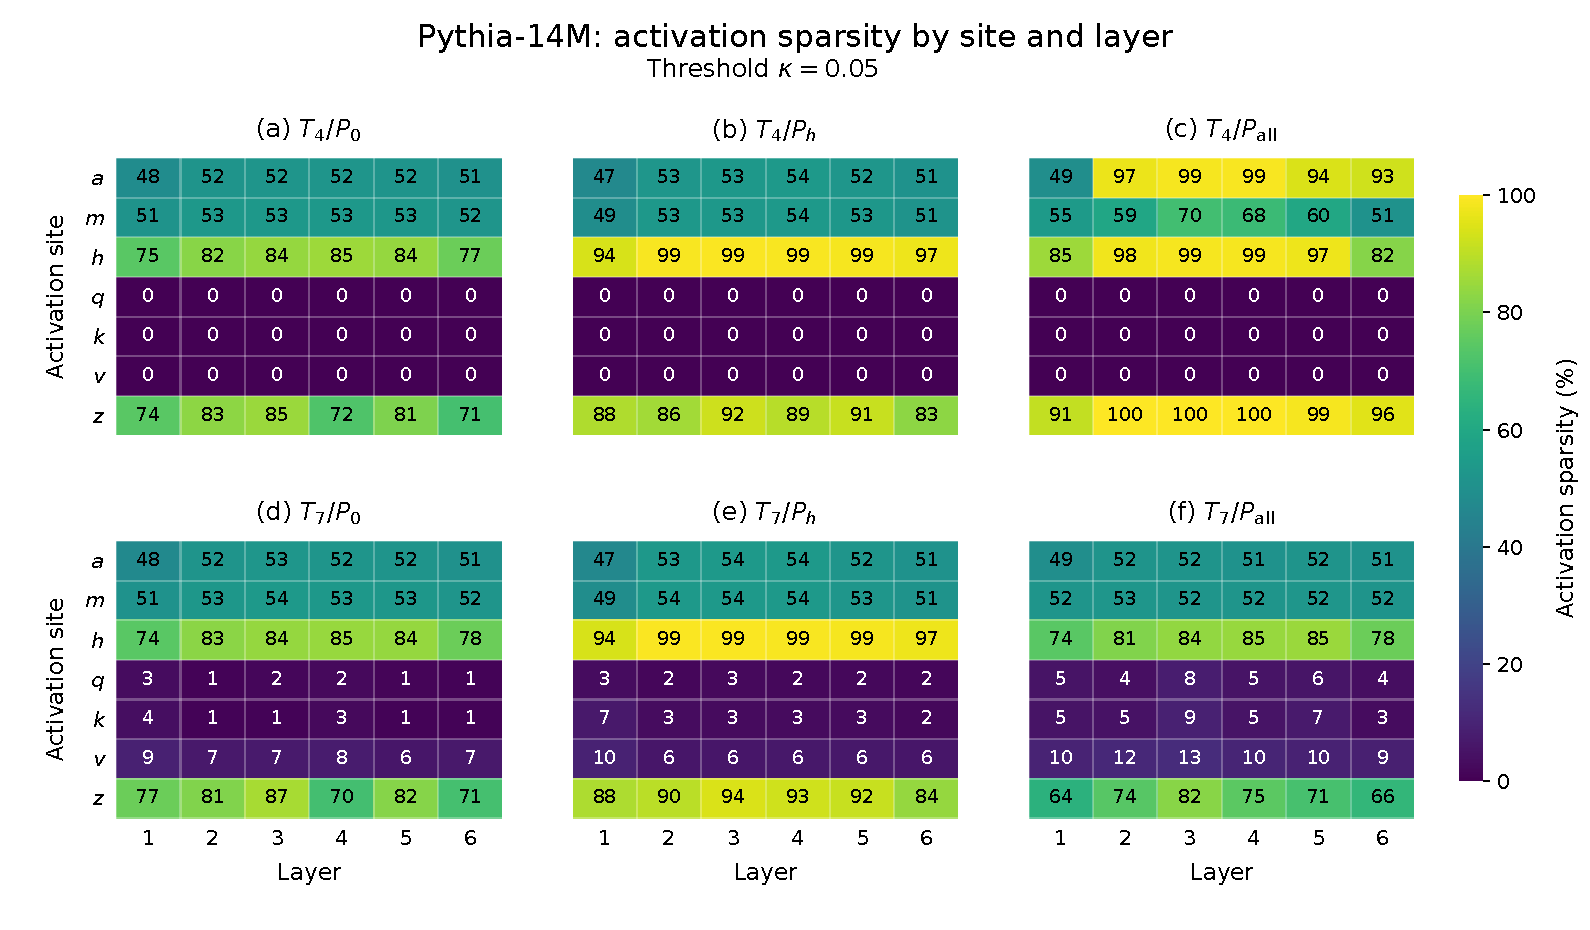
\includegraphics[width=0.9\linewidth,page=1]{figures/appendix-14m-layer-sparsity.pdf}
\caption{\textbf{Activation sparsity by site and layer in Pythia-14M.}
The six threshold/pressure recipes at $\kappa=0.05$: $T_4$ (top) and $T_7$ (bottom), each under $P_0$, $P_h$ and $P_{\mathrm{all}}$.
Each cell gives the percentage of zero activations over all complete validation sequences at one site and layer.
Values are rounded to whole percentages, so 0 or 100 does not establish a completely dense or all-zero tensor.}
\label{fig:pressure-layer-sparsity}
\end{figure}

\textbf{Broader pressure reveals unequal sparse susceptibility across sites.}
Under $T_4/P_{\mathrm{all}}$, extending pressure beyond $h$ increases sparsity across the targeted sites, with $z$ reaching 99.74--99.85\% sparsity in layers 2--4. Extending pressure further under $T_7/P_{\mathrm{all}}$ produces a different pattern: sparsity at $q,k,v$ increases but remains only 3--13\%, while $h$ and $z$ become less sparse than under $P_h$ in every layer. The OL1 geometry in Figure~\ref{fig:ol1-geometry} is consistent with this asymmetry. Pressure outside $h$ produces larger pre-cap correction norms and larger components opposing the task update, and the effect is strongest for $T_7/P_{\mathrm{all}}$. At $\kappa=0.05$, the median removed component rises from 0.15--0.17\% under $P_h$ to 1.12\% for $T_4/P_{\mathrm{all}}$ and 66.84\% for $T_7/P_{\mathrm{all}}$, while the corresponding pre-cap norm ratios rise from 0.08--0.10 to 0.28 and 46.00. Broadening pressure increasingly triggers OL1 projection and norm capping, potentially reducing the effective pressure reaching $h$ and $z$. Together with the spillover effect, these results indicate that $h$ and $z$ are more susceptible to sparsification than the additional sites.

\begin{figure}[!htbp]
\centering
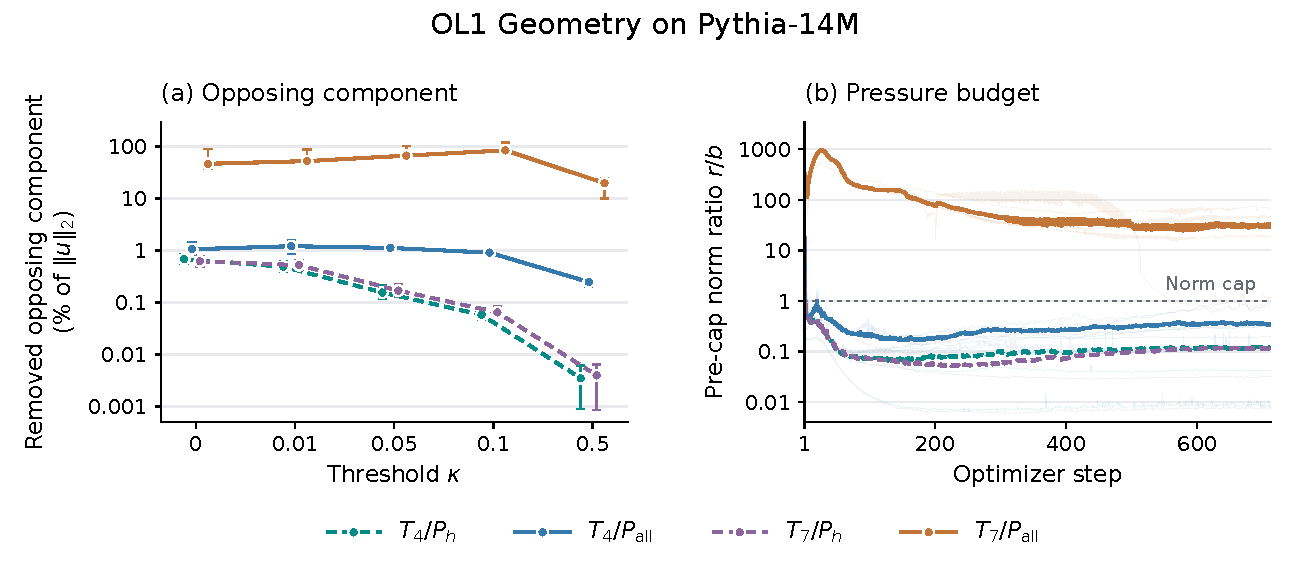
\includegraphics[width=\linewidth]{figures/18-14m-70m-ol1-geometry.pdf}
\caption{\textbf{OL1 geometry depends on pressure placement at 14M.}
\textbf{(a)} Median removed opposing component, $100\rho_{\mathrm{opp}}$;
bars span the 25th--75th percentiles over 712 training steps.
\textbf{(b)} Pre-cap norm ratio $r/b$: bold curves show pointwise
median over individual threshold curves. The dotted line marks the norm cap.}
\label{fig:ol1-geometry}
\end{figure}

\subsection{When sparsity translates to speedup}
\label{sec:activation-reshaping}
\label{sec:kernel-autoresearch}
% Controlled effects: Run037 observations/001-operation-latency.md;
% Analysis024/25_build_operation_latency_table.py; Run039 observations/001-am-port-verdict.md.

We next test whether the sites with the most succeptability to sparsity also respond most strongly to execution time. Table~\ref{tab:kernel-mechanisms} isolates each skipping path at 14M by disabling it while keeping all the other paths fixed. It reports site-sparsity, \emph{bypass} (the percentage of omitted matrix instructions) and conditional saved time for $T_7/P_{\mathrm{all}}$ at $\kappa=0.5$. We test over this recipe because its the sparser variant. The result is aligned with the succeptability observation: \textbf{the measurable savings comes only from $h$ and $z$}.

\begin{table}[!htbp]
\centering\small
\caption{\textbf{Conditional latency savings}: 14M $T_7/P_{\mathrm{all}}$, $\kappa=0.5$.
Latency is measured per 2,048-token sequence on RTX\,5090 (BF16, batch one).
Saved time is full-model latency with one skipping path off minus latency
with all paths on; positive values indicate a benefit (reduced latency).
Brackets give [minimum, maximum] savings across all off/on pairs of three
independent timing runs.
Each run reports the geometric mean over 64 sequences.}
\label{tab:kernel-mechanisms}
% Generated by Analysis024/25_build_operation_latency_table.py.
\setlength{\tabcolsep}{4pt}
\begin{tabular}{@{}lrrrr@{}}
\toprule
Operation & \shortstack{Activation\\sparsity (\%)} & Bypass (\%) & Saved time ($\mu$s) & Process span ($\mu$s) \\
\midrule
$a$: QKV projection & 75.6 & 8.4 & $-1.6$ & $[-6.0, +3.8]$ \\
$m$: FFN-up & 68.6 & 0.0 & $-2.4$ & $[-5.1, +2.7]$ \\
$h$: FFN-down & 99.9 & 94.5 & $+150.1$ & $[+145.4, +154.4]$ \\
$z$: attention-output projection & 99.9 & 99.6 & $+29.0$ & $[+23.7, +35.7]$ \\
$q,k$: $QK$ scores & 93.5 / 94.5 & 58.0 & $-2.9$ & $[-7.3, +1.1]$ \\
$v$: $PV$ product & 98.7 & 67.2 & $-6.2$ & $[-9.0, -2.2]$ \\
\bottomrule
\multicolumn{5}{@{}l@{}}{\footnotesize Activation zeros pooled over layers and validation sequences; $q/k$ reported separately.}
\end{tabular}

\end{table}

Sparsity reduces latency when avoided work exceeds the overhead of detecting and skipping it. At $h,z$, the sparse kernel checks $8\times16$ activation tiles (i.e. sub-matrices)
before loading their associated weights, so empty tiles avoid both weight reads and matrix multiplication. Applying the same strategy at $a$ and $m$ doesn't have an expressive bypass, and instead increased full-model latency by $17.2\%$ and $27.4\%$, because the skipped work does not surpass the additional overhead. We speculate \textbf{that the relation between local sparsity and bypass is not linear, and only over a critical level it translates in a structure that produces high-zero tiles with high probability}.

Attention operations $q,k,v$ follows FlashAttention's tiled computation~\citep{dao2022flashattention}. In our kernel implementation, the zero checks happens only after loading the operands. Skipping a matrix instruction therefore avoids the arithmetic without avoiding those reads and softmax operation. Additionally, softmax turns zero scores into nonzero probabilities, so $q,k$ sparsity does not automatically propagate to $p$. Enabling $qk/pv$ skipping together raises full-model latency from 0.514 to 0.521\,ms despite substantial bypass. So, for this implementation, attention's arithmetic savings do not offset its overhead, while $h/z$ benefit from avoiding weight reads as well as computation.


\subsection{Results at 70M}
\label{sec:quality-sparsity-results}
% Combined figure: Analysis034/observations/002-combined-scales.md; 02_combined.py.
% Claim audit: Analysis034/observations/003-manuscript-integration.md.
% Matched implementations: Analysis028/observations/001-matched-70m-grid.md.

% \textbf{Increasing model size lowers loss but raises latency.}
% %\textbf{Quality vs. latency trade-off accross model sizes.}
% Figure~\ref{fig:70m-quality-latency} compares the 14M and 70M models: native base loss falls from 5.209 to 4.100, while latency rises from 0.655 to 1.611\,ms. For both 14M and 70M, sparse interventions trade quality for lower latency. At aggressive recipes, $T_7/P_{\mathrm{all}}$ at $\kappa=0.5$ increases loss above base by 1.116 at 70M, versus 0.621 at 14M. Yet $T_2/P_h$ retains the lowest loss among the three interventions at every matched $\kappa$. At 70M and $\kappa\leq0.1$, it reaches 14.63--15.21\% model-wide sparsity against a 15.44\% ceiling, with loss 4.129--4.193. \textbf{The concentration of sparsity at $h,z$ with a smaller quality penalty is consistent with their susceptibility extending across the two scales.}

% \textbf{Scaling improves quality but makes aggressive sparsification more costly.}
% Figure~\ref{fig:70m-quality-latency} compares the 14M and 70M models. Scaling to 70M lowers the native loss from 5.209 to 4.100, at the cost of increasing latency from 0.655 to 1.611\,ms. Sparse interventions reduce latency at both scales, but aggressive sparsification incurs a larger quality penalty at 70M: at $\kappa=0.5$, $T_7/P_{\mathrm{all}}$ increases loss above base by 1.116 at 70M, compared with 0.621 at 14M. In contrast, $T_2/P_h$ consistently achieves the lowest loss among the three interventions at matched $\kappa$. At 70M and $\kappa\leq0.1$, it reaches 14.63--15.21\% model-wide sparsity, close to the 15.44\% ceiling, while keeping loss between 4.129 and 4.193. \textbf{This persistence of concentrated sparsity at $h,z$ with a smaller quality penalty suggests that their susceptibility extends across model scales.}


\textbf{Scaling improves quality and amplifies the latency payoff of targeted sparsification.}
Figure~\ref{fig:70m-quality-latency} compares the 14M and 70M models. Scaling to 70M lowers native loss from 5.209 to 4.100, while increasing latency from 0.655 to 1.611\,ms. Sparse interventions reduce latency at both scales, but aggressive recipes takes a larger quality penalty at 70M: at $\kappa=0.5$, $T_7/P_{\mathrm{all}}$ loss increases above base by 1.116 at 70M, versus 0.621 at 14M. In contrast, $T_2/P_h$ consistently achieves the lowest loss among the tested interventions at matched $\kappa$, reaching 14.63--15.21\% model-wide sparsity at 70M for $\kappa\leq0.1$, close to the 15.44\% ceiling. Increasing $\kappa$ from 0 to 0.1 reduces latency by 0.039\,ms at 14M but by 0.549\,ms at 70M; increasing it further to 0.5 yields another 0.741\,ms reduction at 70M, at the cost of increasing loss from 4.182 to 4.838. The sharp transition between $\kappa=0.1$ and $0.5$ motivates testing intermediate thresholds at $h,z$. Overall, targeted sparsity at $h,z$ remains effective across scales, while its latency benefit grows substantially with model size.


\begin{figure}[!htbp]
\centering
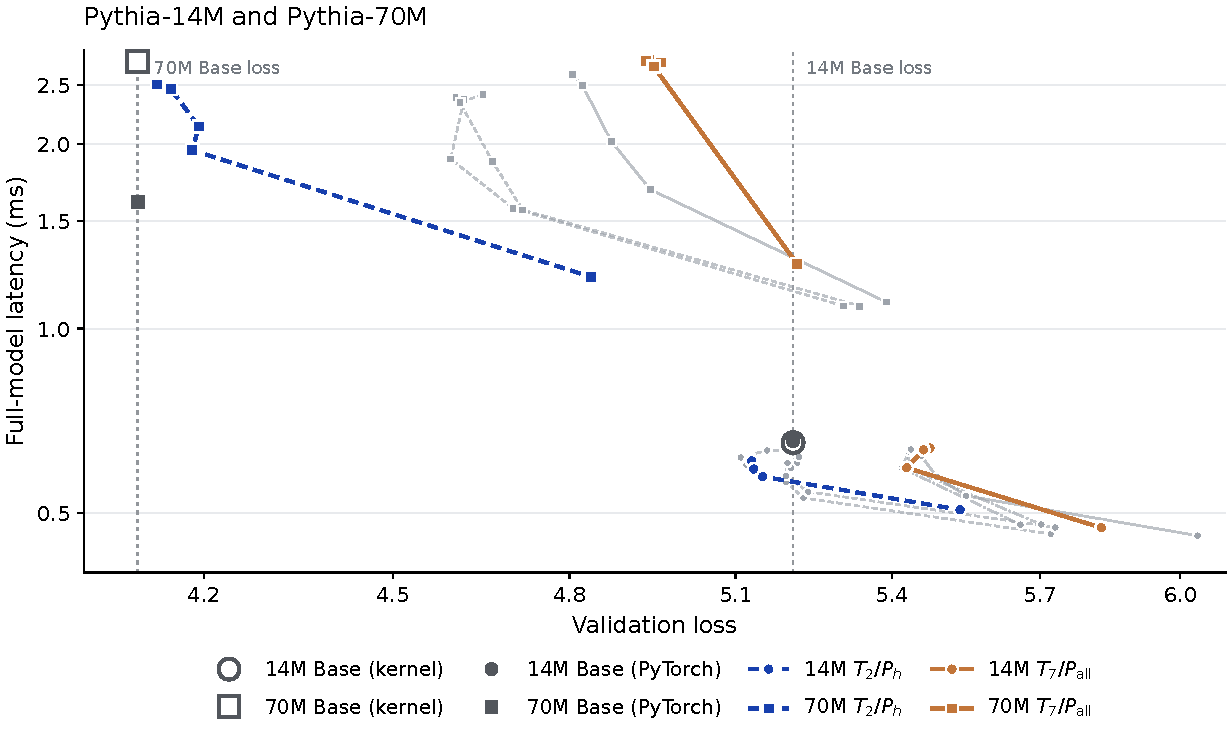
\includegraphics[width=\linewidth]{figures/02-14m-70m-latency-quality.pdf}
\caption{\textbf{Validation loss and full-model latency across model sizes.}
Circles denote 14M and squares 70M; $T_2/P_h$ is blue, $T_7/P_{\mathrm{all}}$ orange, and other recipes gray. Lines connect settings within each recipe and size. Both axes are logarithmic. Each Base checkpoint appears under kernel and native PyTorch execution; vertical guides mark Base loss. The 64 intervention points use the specialized kernels for their respective sizes. Timings use RTX\,5090, BF16, batch one, 2,048 tokens and full logits.}
\label{fig:70m-quality-latency}
\end{figure}

% \textbf{Threshold strength controls trade-off at both scales.}
% For $T_2/P_h$, increasing $\kappa$ from 0 to 0.1 reduces latency from 0.612 to 0.573\,ms at 14M (0.039\,ms), and from 2.504 to 1.956\,ms at 70M (0.549\,ms). Increasing $\kappa$ further to 0.5 brings 70M latency to 1.214\,ms (a further 0.741\,ms reduction) but raises loss from 4.182 to 4.838. The large gap between $\kappa\in\{0.1,0.5\}$ motivates further testing of intermediate thresholds at $h,z$. The corresponding latency reduction from $\kappa=0.1$ to 0.5 at 14M is 0.067\,ms, so the absolute reduction at 70M is $11.0\times$ as large (Table~\ref{tab:endpoints-14m-70m} provides the full comparison). \textbf{This is evidence of exploitable sparse structure at both scales}.

However, \textbf{the 14M kernel does not transfer efficiently to 70M.}
On the 70M base model, adapting the 14M kernel to the larger dimensions yields 3.325\,ms latency, compared with 1.611\,ms for native PyTorch (overhead of 1.714\,ms for the dense execution). A further optimization pass improves sparse $h,z$ execution and dense components, reducing Base latency to 2.732\,ms, but still leaving a 1.121\,ms gap. The fastest sparse recipe, $T_7/P_h$ at $\kappa=0.5$, reaches 1.088\,ms, 32.5\% below native Base, but at a substantial quality cost: its loss increases by 1.237 to 5.337. These results show that useful sparse structure persists at 70M, but the kernel implementation requires further optimization even within the same model family. The gains from our partial re-optimization also indicate remaining kernel-level headroom, but our current implementation does not yet exploit it without requiring aggressive sparsification.


% % Controlled 70M evidence: Analysis028/04_controls.py and data/retained-controls.json.
% \textbf{Sparse execution remains useful, but its implementation requires adaptation.}
% In a separate session on the same 70M $T_7/P_h$ checkpoint at $\kappa=0.5$, replacing only the specialized $h,z$ path with native operations raises latency from 1.128 to 1.365\,ms: a conditional 0.237\,ms (17.4\%) benefit from the specialized path, including fusion and layout effects. The corresponding skip-disabled control is reported in Appendix~\ref{app:kernel-transfer}. Thus, useful sparse structure can persist while kernel efficiency fails to transfer, even within one model family. Our results motivate kernels adapted to model size and workload, rather than assuming that a published implementation transfers unchanged. Training interventions and kernel execution must therefore be co-designed: training should induce sparse structures that the target kernel can exploit at an acceptable quality cost.

% \subsection{Failures and Limitations}
% Limitation: We limited the scaling analysis to 14M and 70M. Justification: We also evaluated 410M, but it operates in a different optimization regime, with higher loss than 70M and a larger gradient norm after the same token budget (Appendix~\ref{app:410m-results}).
% Limitation: Kernel efficiency does not transferred directly across scales. Justification: we tried optimizing it, got a better result.. but didn't converged on a better solution.
% Limitation: runtime measurements are restricted to batch-one, full-sequence inference on a single GPU. Justification: simple enough for a train-time intervention experiment.
% Limitation: Training comparisons use one seed per condition. Justification: we have a well-behaved relation accross recipes and ran dozens of variants accross methods. We understand there is randomness on point-results.. but since the trade-offs accross recipes are well-behaved, we take it as evidence.
% Finally, the intervention space is combinatorial: we study only selected placements, and broad-pressure ablations change several sites jointly rather than isolating each site's contribution. Justification: future results can isolate pressure accross single sites, eliminate the OL1 averaging accross sites cofound, work with different thresholds accross sites.




\FloatBarrier




%\subsection{Paired effects of global vs. local pressure}




% \textbf{Threshold strength changes which sites remain responsive to pressure.}
% At $\kappa=0.5$, $h$ and $z$ already round to 100\% sparsity without pressure, whereas under $T_7/P_0$ the other sites remain substantially denser: $a,m$ lie between 57--70\%, and $q,k,v$ between 13--36\%.
% Broad pressure then primarily increases sparsity at these remaining sites rather than at the already saturated $h$ and $z$ activations.
% The strong site dependence in Figure~\ref{fig:pressure-layer-sparsity} motivates asking whether sparsity at different locations also differs in its value for execution.


% % Source: analyses/024-2026-09-17-h-only-kernel-latency/observations/015-pressure-scope-caption.md;
% % generating analysis: paper_effect_figures.py / 13_rebuild_paper_figures.py;
% % adoption and checked claims: manuscript/draft/reviews/2026-09-18-paired-pressure/README.md.
% One question raised during sparse intervention design is wheater \textbf{activation pressure should be applied over the entire network, or are there local sites more suceptible to sparsification?} To answer this, we compare thresholding accross multiple sites ($T_4$ and $T_7$) with global and local FFN hidden pressure ($P_{all}$ and $P_h$) at Figure~\ref{fig:paired-intervention-effects}.

% \begin{figure}[!htbp]
% \centering
% 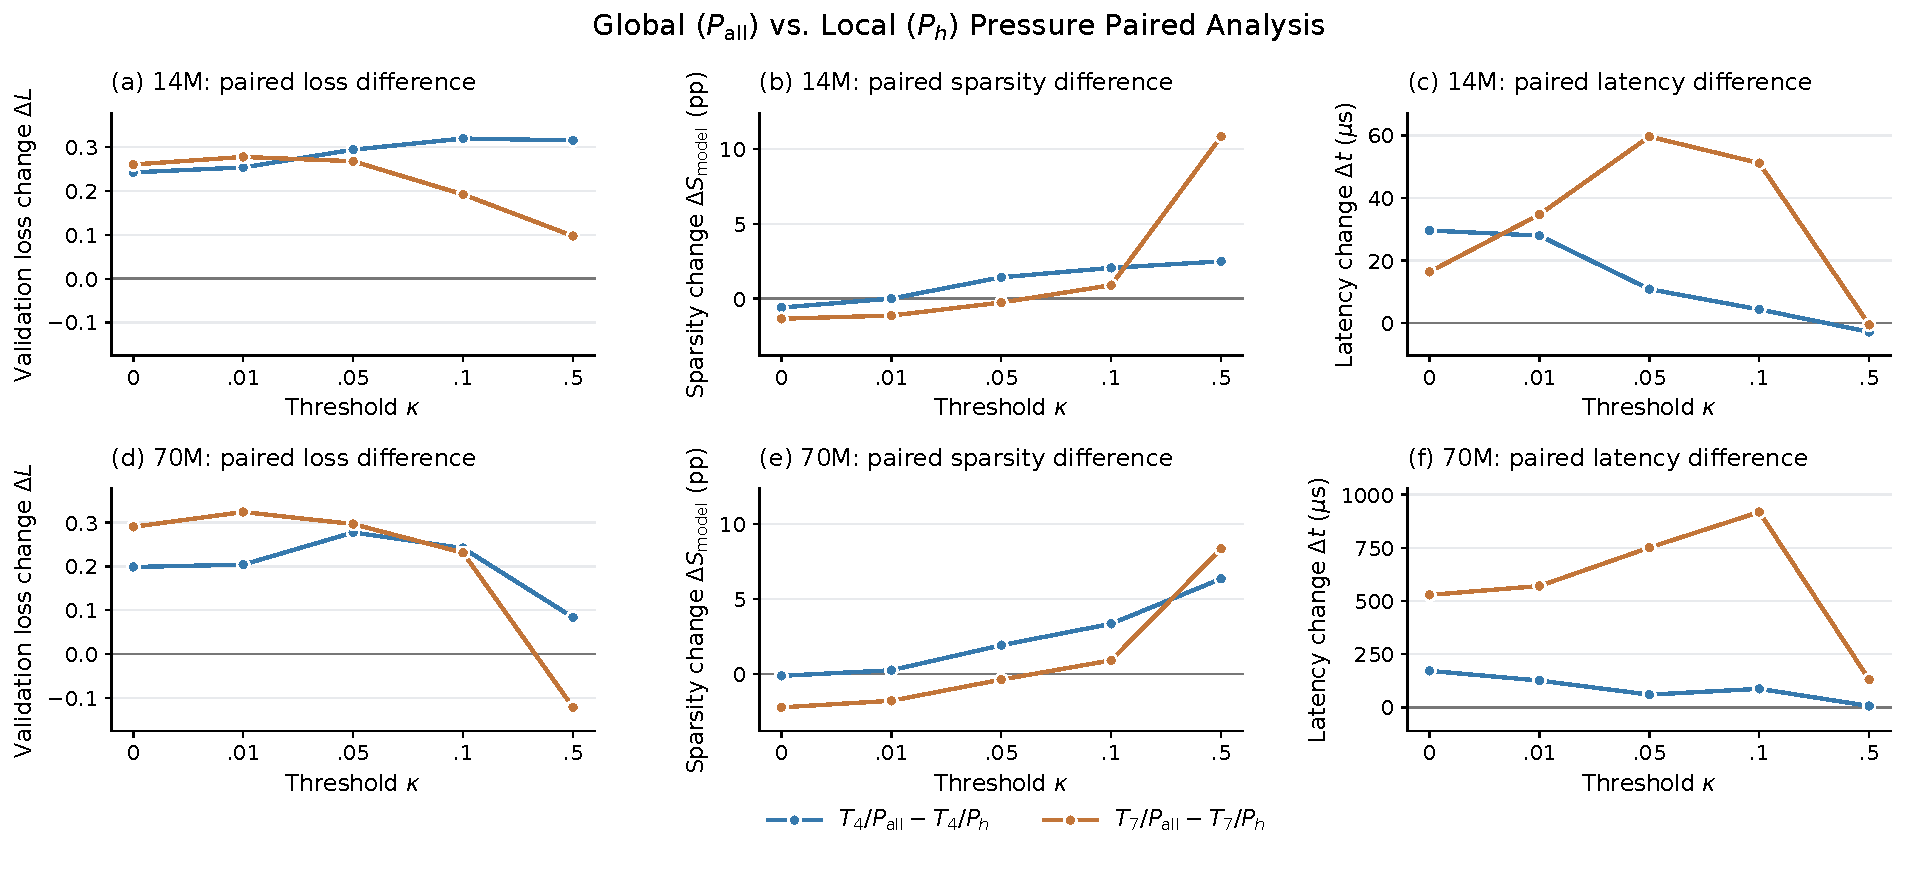
\includegraphics[width=\linewidth]{figures/03-pressure-scope-threshold.pdf}
% \caption{\textbf{Paired effects of broadening pressure from $P_h$ to $P_{\mathrm{all}}$.}
% Every point is $P_{all}$ minus $P_h$ at matched model size, threshold sites and $\kappa$, with $\lambda=b=1$. Rows show 14M/70M; columns show loss change, sparsity change (pp), and full-model latency change ($\mu$s).
% Positive loss or latency differences favor $P_h$; positive sparsity differences favor $P_{\mathrm{all}}$.
% }
% \label{fig:paired-intervention-effects}
% \end{figure}


% \textbf{Global pressure achieves higher sparsity at a greater quality cost, without translating this additional sparsity into lower latency.} At moderate thresholds ($\kappa\leq0.1$), local h-only pressure ($P_h$) provides a more favorable quality--sparsity trade-off than global pressure ($P_{\mathrm{all}}$) in both model sizes: $P_h$ lowers loss in all 16 matched comparisons at 14M and 70M (Figure~\ref{fig:paired-intervention-effects}), with reductions of $0.19$--$0.32$ while sparsity differs by at most $3.36$ percentage points. Although broader pressure can achieve higher sparsity, this gain does not translate into lower measured latency: h-only pressure is faster in 18 of the 20 matched pairs, including all ten 70M pairs. Thus, applying sparsity pressure globally trades model quality for additional sparsity without yielding a corresponding inference-time benefit.


% % \textbf{Local h-only pressure gives a more favorable quality--sparsity trade-off at moderate thresholds in both model sizes}.
% % For $\kappa\leq0.1$, $P_h$ lowers loss relative to $P_{\mathrm{all}}$ in all 16 matched comparisons at 14M and 70M
% % (Figure~\ref{fig:paired-intervention-effects}). The loss reduction is $0.19$--$0.32$, with sparsity differing by at most $3.36$ percentage points.
% % % At $\kappa=0.5$, all-site pressure instead gives substantially more sparsity,
% % % especially for $T_7$; at 70M it also lowers the $T_7$ loss by $0.121$.

% % \textbf{The additional sparsity from global pressure does not imply in lower latency}. H-only pressure has lower measured latency in 18 of the 20 pairs, including all ten 70M pairs.
% % % The two small reversals occur at 14M and $\kappa=0.5$: all-site pressure is faster by $2.78\,\mu$s for $T_4$ and $0.52\,\mu$s for $T_7$.
% % Thus, the extra sparsity from broader pressure does not consistently translate into lower latency.


% % Source: Analysis021 pressure-scope/observations/O016-pressure-placement.md
% % and O017-layer-sparsity-style.md; figure: pressure-scope/plot_layer_sparsity.py.
% \textbf{Local pressure can produce nonlocal sparsity changes}. Figure~\ref{fig:pressure-layer-sparsity} present the sparsity by site and layer accross $T_4$ and $T_7$ interventions, for all pressures at 14M. At $\kappa=0.05$, $P_h$ increases sparsity at both $h$ and $z$ relative to $P_0$, although $z$ receives no direct pressure. Under $T_7$, $P_h$ also produces higher sparsity at $h$ and $z$ than $P_{\mathrm{all}}$, despite the latter targeting both sites. One possible explanation is that (q,k,v) increases $\ell_1$ pressure norms, and $P_{all}$ caps the OL1 norm more frequently (Appendix~\ref{app:pressure-budget-diagnostics}), reducing the local at $h$. The takeaway is that a local site pressure may spillover and affect the distributions of other sites.

% \begin{figure}[H]
% \centering
% 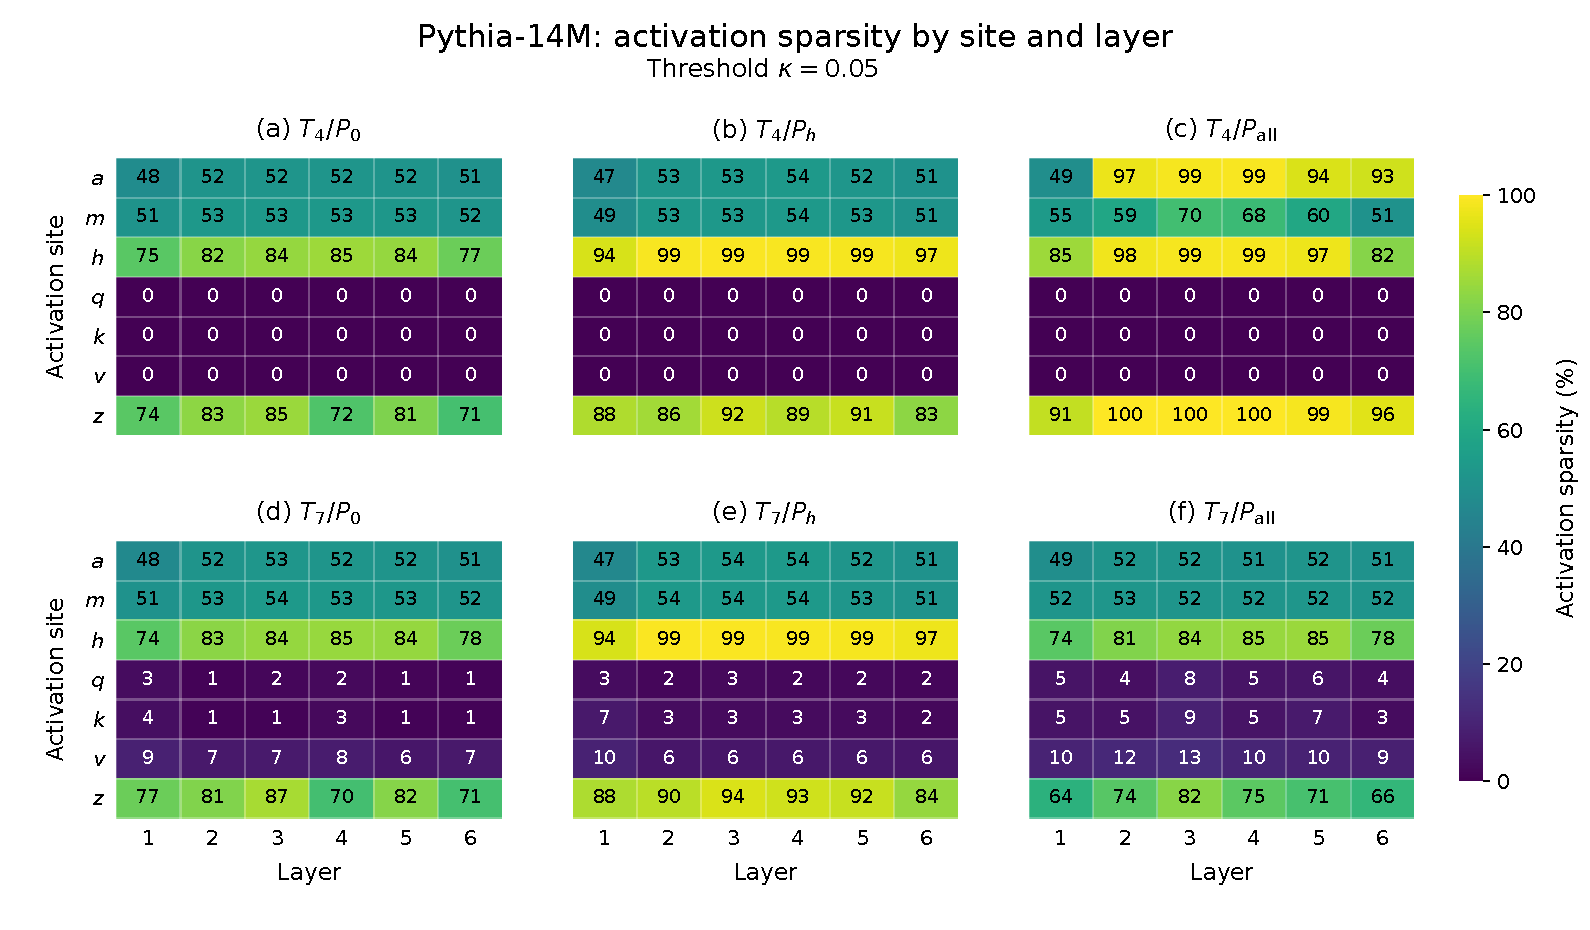
\includegraphics[width=0.9\linewidth,page=1]{figures/appendix-14m-layer-sparsity.pdf}
% \includegraphics[width=0.9\linewidth,page=2]{figures/appendix-14m-layer-sparsity.pdf}
% \caption{\textbf{Activation sparsity by site and layer in Pythia-14M.}
% The six threshold/pressure recipes at $\kappa=0.05$ (top) and $0.5$ (bottom).
% Each cell gives the percentage of zero activations over all complete validation sequences at one site and layer.
% Q/K are post-RoPE; all panels share a 0--100\% color scale.
% Values are rounded to whole percentages, so 0 or 100 does not establish a completely dense or all-zero tensor.}
% \label{fig:pressure-layer-sparsity}
% \end{figure}

% \textbf{(h, z) are more succeptible to sparsification}. At higher threshold ($\kappa=0.5$) (h,z) sites become fully sparse, even if no pressure is applied; while (q,k,v) sites are in the $[14, 36]$ and (a,m) are in $[57,70]$ sparsity range. This implies the distribution of (q,k,v) and (a,m) may have different ranges and require different threshold values than (h,z).

% \FloatBarrier

%% Evidence: Analysis024 observations/034-operation-latency-manuscript.md;
% Run037 observations/001-operation-latency.md and results/conditional-effects-audit.json.
% Table generator: Analysis024/25_build_operation_latency_table.py.
% a/m port evidence: Analysis024 observations/035-am-load-avoidance-port.md;
% Run039 observations/001-am-port-verdict.md, results/am-load-avoidance.json
% and results/mechanism.json; reducers: Run039/07_reduce.py and 12_mechanism.py.
% Mechanism: Run028 candidates/k049/joint.cu, k042/projection.cu,
% k035/sparse_gemm.h and k035/flash_fwd_kernel.h; Run029 implementation audit.
\subsection{When model-wide sparsity translates to speedup}
\label{sec:activation-reshaping}
\label{sec:kernel-autoresearch}

Sparsity reduces latency when avoided work exceeds the cost of detecting and
skipping zeros. At $h,z$, our kernel checks $8\times16$ activation groups
before loading their weights: empty groups avoid both weight reads and matrix
multiplications. At $a,m$, the $16\times16$ checks occur after both operands
are loaded, so skipping saves only arithmetic.
A follow-up test supports this choice: applying the $h/z$ strategy separately
at $a$ and $m$ increased full-model latency by $17.2\%$ and $27.4\%$ on
14M $T_7/P_{\mathrm{all}}$ at $\kappa=0.5$, with unchanged outputs.
Only $11.12\%$ of $a$'s $8\times16$ tiles were empty, and none at $m$, so
most groups still required matrix multiplication. Padding eight real rows to
sixteen-row matrix instructions increased issued instructions by $1.90\times$
at $a$ and $2\times$ at $m$. At $h/z$, most rows instead have at most two
nonzero activations, making the cheaper scalar path useful much more often.

Attention follows FlashAttention's tiled sequence \citep{dao2022flashattention}:
load $Q,K$, compute scores, apply masking and softmax, then multiply
probabilities by $V$. Our checks occur after operand loads; skipping an empty
tile's multiplication cannot recover those reads. Softmax still runs and
turns zero scores into nonzero probabilities, so $Q/K$ sparsity does not
automatically propagate to $PV$. Zeros in $V$ remain usable; sparsifying the
probabilities is a further opportunity, untested here.

We isolate each path's effect at 14M by disabling it while holding weights,
gates and all other skipping paths fixed (Table~\ref{tab:kernel-mechanisms}).
\emph{Bypass} counts skipped matrix instructions divided by issued plus
skipped instructions; it does not measure the fraction of runtime saved.

\begin{table}[!htbp]
\centering\small
\caption{\textbf{Conditional latency savings: 14M $T_7/P_{\mathrm{all}}$, $\kappa=0.5$.}
Times are per 2,048-token sequence on RTX\,5090 (BF16, batch one).
Saved time is full-model latency with one skipping path off minus latency
with all paths on; positive values indicate a benefit.
Brackets give [minimum, maximum] savings across all off/on pairs of three
independent timing runs per mode, not confidence intervals.
Each run reports the geometric mean over 64 sequences and seven passes.
Effects are not additive.}
\label{tab:kernel-mechanisms}
% Generated by Analysis024/25_build_operation_latency_table.py.
\begin{tabular}{@{}lrrr@{}}
\toprule
Operation & Bypass (\%) & Saved time ($\mu$s) & Process span ($\mu$s) \\
\midrule
$a$: QKV projection & 8.4 & $-1.6$ & $[-6.0, +3.8]$ \\
$m$: FFN-up & 0.0 & $-2.4$ & $[-5.1, +2.7]$ \\
$h$: FFN-down & 94.5 & $+150.1$ & $[+145.4, +154.4]$ \\
$z$: attention-output projection & 99.6 & $+29.0$ & $[+23.7, +35.7]$ \\
$q,k$: $QK$ scores & 58.0 & $-2.9$ & $[-7.3, +1.1]$ \\
$v$: $PV$ product & 67.2 & $-6.2$ & $[-9.0, -2.2]$ \\
\bottomrule
\end{tabular}

\end{table}

The clear savings come from $h$ ($150\,\mu$s) and $z$ ($29\,\mu$s).
Individual $a,m,QK$ effects remain unresolved against process variation,
whereas $PV$ skipping adds latency. Enabling $QK/PV$ skipping together raises
full-model latency from 0.514 to 0.521\,ms despite substantial bypass.
Thus, for this checkpoint and implementation, attention's arithmetic savings
do not offset its overhead, while $h/z$ benefit from avoiding weight reads
as well as computation.

\FloatBarrier

